%!TEX TS-program = pdflatex

\documentclass[nocopyrightspace,10pt]{sigplanconf}
\usepackage{hyperref}
\usepackage{xspace}
\usepackage{textcomp}
\usepackage{graphicx}

\setlength{\columnsep}{4em}

\begin{document}

\title{The ``Who's Yo Daddy?'' Problem \\ \Large{Or: Solvin' Concurren' Axcess Issues wit Computers, Yo}}

\authorinfo{Dr. Donna M. Malayeri, PhD}{}{}
\authorinfo{Heather Miller, PhD(c), Esq., PPPoE, P2P}{}{}          
\authorinfo{Herr Doctor Doktor Klaus Haller}{}{}
\date{April 1, 2011}

\nocaptionrule

\maketitle

\pagestyle{empty}
\thispagestyle{empty}

\begin{abstract}
Computer Science research can solve many real-world problems. Here we describe our novel research, Uniqueness Types, and how it applies both to multi-threaded programs and to real world scenarios. In particular, we solve issues that commonly arise in popular daytime sociological science documentaries.\footnote{E.g., \emph{The Jerry Springer Show}.}
\end{abstract}

\section{Introduction}
In multi-threaded programs resources such as memory and files are at the same time accessed, i.e., concurrently. This often leads to problems, such as blue screens, not-disappearing hour glasses, the spinning dying color wheel of death and so forth. For example, let's consider a thread program that a file opens, and it accesses. It may happen that yet another threaded process at some later point in time closes the file without the first program knowing about it. If the first program to the file again accesses, then the user may a blue screen experience.

\section{Uniqueness Types}
To solve the unique problems introduced in the introduction, we introduce a novel language-theoretic type theory called Uniqueness Types \cite{philipp}. We base our theoretical theory on flow-sensitive linear logic with typestate~\cite{kevin}. The idea of our research approach is to assign unique types to pointer variables. A pointer is unique whenever the compiler program knows that all other pointers are pointing towards other datums, or, conversely, if and only if no other pointer is pointing towards it. In predated works computer researchers have published theoretical experiments with unique pointers that sometimes their typestates change.

Unique pointers with uniqueness types give rise to a unique approach to avoid the unique problems of hour glasses and spinning dying color wheel of death. Somehow we can make sure everyone points to the hour glass or something like that. Or no, maybe the thread program must have pointers with unique names.\footnote{Americanadian translation: if two threads access the same resource, say a file, it would be bad if one thread opened the file, then the other thread closed the file, then the first thread tried to then read from the file. Essentially, threads with pointers to a shared resource need to know about state changes that may affect future operations on that resource. A uniqueness type solves this problem, and you can read more about it in this boring---er, exciting---research paper \cite{philipp}.}

\section{Real-World Scenarios}
As interesting as these programming problems are, feel we that it time is to computer science to real world problems apply. How else can we, with a straight face, to funding agencies the claim make that we real problems that affect people's everyday lives solve?

We believe that a good source of real-world problems documentaries is, particularly those highly-rated ones that on broadcast television are shown. These informational programs an unprecedented view into the daily life of the everyman provide. For the purposes of this paper, \emph{The Jerry Springer Show} as our primary source we shall use, though our solution to scenarios seen on other esteemed programs is applicable, such as \emph{The Maury Povich Show} or \emph{Jersey Shore}.

\subsection{Real-World Problem Statement}

\begin{quote}
So, this one bitch is a real ho fo real and she get wit three playaz, Playa 1, Playa II, and Playa Playaa Playa. And now showty pregnan' and she sez the baby daddy is Playa Playaa Playa and he a pimp.\footnote{This means he has lots of money.} He sho' Playa 1 is da baby daddy fo serious and he don wants to pay no child suppo'. Da ho gots a paternity test dat sez da baby daddy is Play Playaa Playa but he thank it a fake.
\end{quote}

Here, the problem is access to the shared resource within a critical timeframe. Since the third man does not trust the results of the paternity test, believing the woman to be a ``lyin' ho,'' we need to provide the parties in this scenario with a fool-proof mechanism for determining parentage.

We believe this problem is widespread, and in the tradition of clever monikers for computer science problems (e.g., Travelling Salesman, Sleeping Barber, Dining Philosophers), we name this problem ``Who's Your Daddy?''

Further, this is a problem that clearly arises often in practice. As evidence, see Figures~\ref{fig:kittens},~\ref{fig:springer}, and~\ref{fig:jersey}.

\begin{figure}[tbh!]
\centering
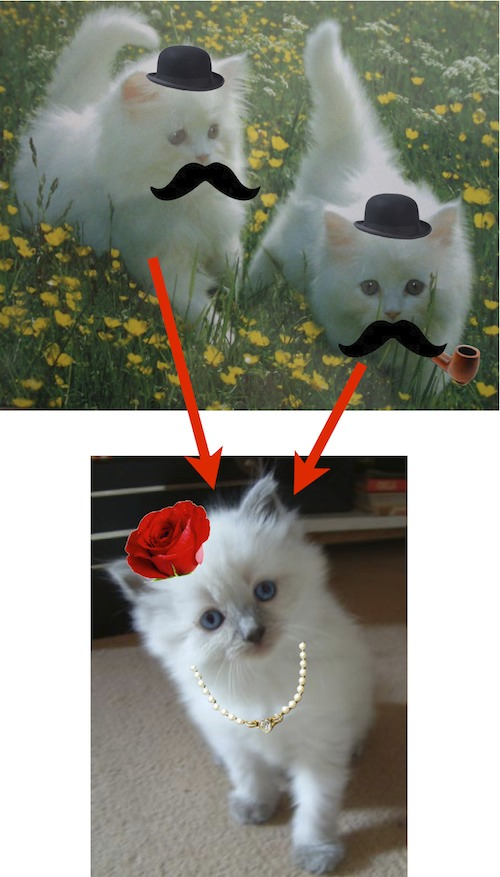
\includegraphics[width=0.9\linewidth]{kittens.jpg}
\caption{Two male kittens access a shared female kitten resource, creating contention. (No, this is not a gratuitous kitten picture.)}
\label{fig:kittens}
\end{figure}

\begin{figure}[tbh!]
\centering

\includegraphics[width=\linewidth]{jerry-springer.jpg}
\caption{Unexpected physical confrontation of two threads who accessed a female within the same timeframe.}
\label{fig:springer}
\end{figure}

\begin{figure}[tbh!]
\centering

\includegraphics[width=\linewidth]{jersey-shore.jpg}
\caption{The shared resource unsuccessfully attempts to arbitrate between threads who are engaged in a violent altercation. As seen on \emph{Jersey Shore}.}
\label{fig:jersey}
\end{figure}


\section{Applicability to Real-World Scenarios}
It is not immediately obvious how the theoretical results of Uniqueness Types to Who's Your Daddy can be applied. We present here an iterative approach to a solution, starting with a na\"{i}ve solution and refining it to handle all possible scenarios.

\subsection{Solution 1: H\"{e}\"{a}vy \"{M}\"{e}t\"{a}l Locking Device with Physical Key}
The problem here is that several pointers the shared resource may access, and her state may at any time change, without it being obvious to any of the parties involved (including the resource herself) that a) the state change has occurred and b) which pointer caused the state change.

We introduce the following protocol:
\begin{itemize}
\item An external party outfits the resource with a h\"{e}\"{a}vy \"{m}\"{e}t\"{a}l locking device with a physical key. For instance, the Victorian chastity belt would be quite useful here (Fig.~\ref{fig:chastity}).
\item The physical key is retained by the external party for an incubation period of not less than 9 months.
\item The first pointer retrieves the key from the external party and may access the resource.
\item When the first pointer is finished with the resource, he or she returns the key to the external party.
\item The incubation period is again started and the process repeats itself.
\end{itemize}

\begin{figure}[tbh!]
\centering
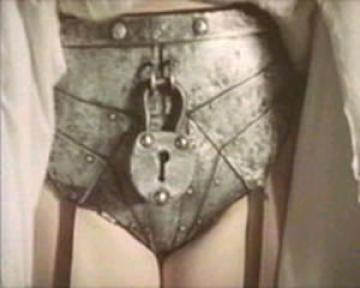
\includegraphics[width=0.75\linewidth]{chastity-belt2.jpg}
\caption{An antique h\"{e}\"{a}vy \"{m}\"{e}t\"{a}l locking device. Note that this version lacks many of the features required in our solution, and is therefore far inferior to our proposed locking device.}
\label{fig:chastity}
\end{figure}

However, this na\"{i}ve approach is fraught with issues. The pointer who has the key in his or her possession may initiate an ownership transfer, either wanted or unwanted (i.e., in cases of theft). Moreover, borrowing re-introduces the same race condition that the protocol had attempted to eliminate. Thus, anyone with a copy of the key to the h\"{e}\"{a}vy \"{m}\"{e}t\"{a}l locking device may be the future Baby Daddy, which again leaves the question unresolved: Who's Your Daddy?

\subsection{Solution 2: H\"{e}\"{a}vy \"{M}\"{e}t\"{a}l Locking Device with Biometric Key}
This solution is similar to the first, except the pointer is the access key. However, this means that once a particular pointer has accessed the resource, she may henceforth never be accessed by any other pointer. This is problematic if the first pointer gets bored and leaves, or is otherwise destroyed.

\subsection{Solution 3: H\"{e}\"{a}vy \"{M}\"{e}t\"{a}l Locking Device with Dynamic Biometric Key, aka She Crimped A Ladysman AndShit (SCALA)}
This is similar to Solution 2, except now the locking device can be re-keyed by the external party to any particular pointer, assuming that the resource is in the vacant state (which can always be determined once the incubation period has passed).

\subsubsection{Translation to Lay Speak}
Now, dis shit gettin' futuristic and shit yo. Now, to get wit dis bitch, you gots to go to her mama and daddy and get permission and shit. If she ain't wit nobody and she ain't pregan' then they crimp yo junk in computer shit an make it so no other playa get in dem locked panties and shit. Na'i mean? That shit mothafuckin sucks, brace yoself foo' cuz dat shit mothafuckin stings an dey know it was you when shit happen.

\subsection{SCALA Solves Everything}
The solution is clearly SCALA\footnote{She Crimped A Ladysman AndShit} with Uniqueness Types. We draw here on previous work which also considered the urban implications of SCALA \cite{pimp-my-library}.

\section{Conclusions and Future Work}
We have shown that research that problems in multi-threaded programs solves can also to serious real-world scenarios be applied. With a minor modification to existing technology (the metal locking device), have we demonstrated how to solve a wide array of problems in popular socio-scientific documentaries seen. In particular, with our solution, can we always definitively that key question answer, ``Who's Yo Daddy?''

\vspace{2ex}

Yo so this is the mothafuckin straight deal yo. Dey take da shit dey do on computers and shit and fuckin make it so yo badonkadonkical ho can't gets with no otha balla. So when she sez you da baby daddy you jus gotta say to the otha playa, ``Drop yo draws boy I know yo junk be crimped.''

\section{Acknowledgements}
Herr Doctor Doktor Klaus provided all of the middle-English-like sentences. The other authors thank him highly for this immense contribution, which would not be possible without a native German speaker. Ebonics translation gracefully provided by Frau Hezza (aka Hedair). Thanks greatly to the fucking wild input from Dr.~Jenn~B.~S.

\footnotesize{
\begin{thebibliography}{50}
\bibitem{kevin} Bierhoff, Kevin, Nels E. Beckman and Jonathan Aldrich. Practical API Protocol Checking with Access Permissions. In \emph{23rd European Conference on Object-Oriented Programming (ECOOP)}, 2009.

\bibitem{philipp} Haller, Philipp and Martin Odersky. Capabilities for Uniqueness and Borrowing. In \emph{24th European Conference on Object-Oriented Programming (ECOOP)}, 2010.

\bibitem{pimp-my-library} PhD, Malayeri, Donna Dr. ``Pimp My Library'' Is An Affront To Pimpers Of The World, Everywhere. In \emph{Proceedings of SIGBOVK 2010}, Pittsburgh, PA, USA, 2010.


\end{thebibliography}
}

\end{document}